\section{Introduction to EU's Artificial Intelligence Act: The European Approach to AI}
    In order to understand the research project and the associated system for automatic and predictive traffic guidance of the Fraunhofer Institute in detail, a general look at the European Commission's draft of the EU Artificial Intelligence Act will be discussed beforehand.\\
    On April 21, 2021, the European Commission presented its proposal for a regulation that would provide harmonized rules for the use and management of artificial intelligence (AI) in the EU - in short, the AI Act. The draft regulation aims to standardize the approach to AI and, in particular, to align it with the EU's high standards of trustworthy AI. [\citet{kop2021eu}]. The proposed Regulation sets out fundamental rules for the development, commercialization, and utilization of AI-driven products, services, and systems in the territory of the EU, applicable to all industries. For the implementation of this, a system based on four risk categories has been developed, which sets different compliance rules at the respective risk levels. [\citet{ebers2021standardizing}] The AI Act suggests categorizing AI systems into four levels of risk based on threats to health, safety, and constitutional rights, 1. unacceptable, 2. high, 3. limited, and 4. minimal.  [\citet{lutge2022risk}] This risk-based approach based on the criticality pyramid (see below) is combined with a sophisticated, multi-level regulatory enforcement mechanism. As a result, stricter rules apply as the risk increases. AI systems that pose unacceptable risk are prohibited, high-risk AI systems face a long list of pre-market and post-market requirements. Limited-risk AI systems are governed by transparency obligations, and minimal- to no-risk AI systems can be used liberally.\\

    \begin{figure}[h]
        \centering
        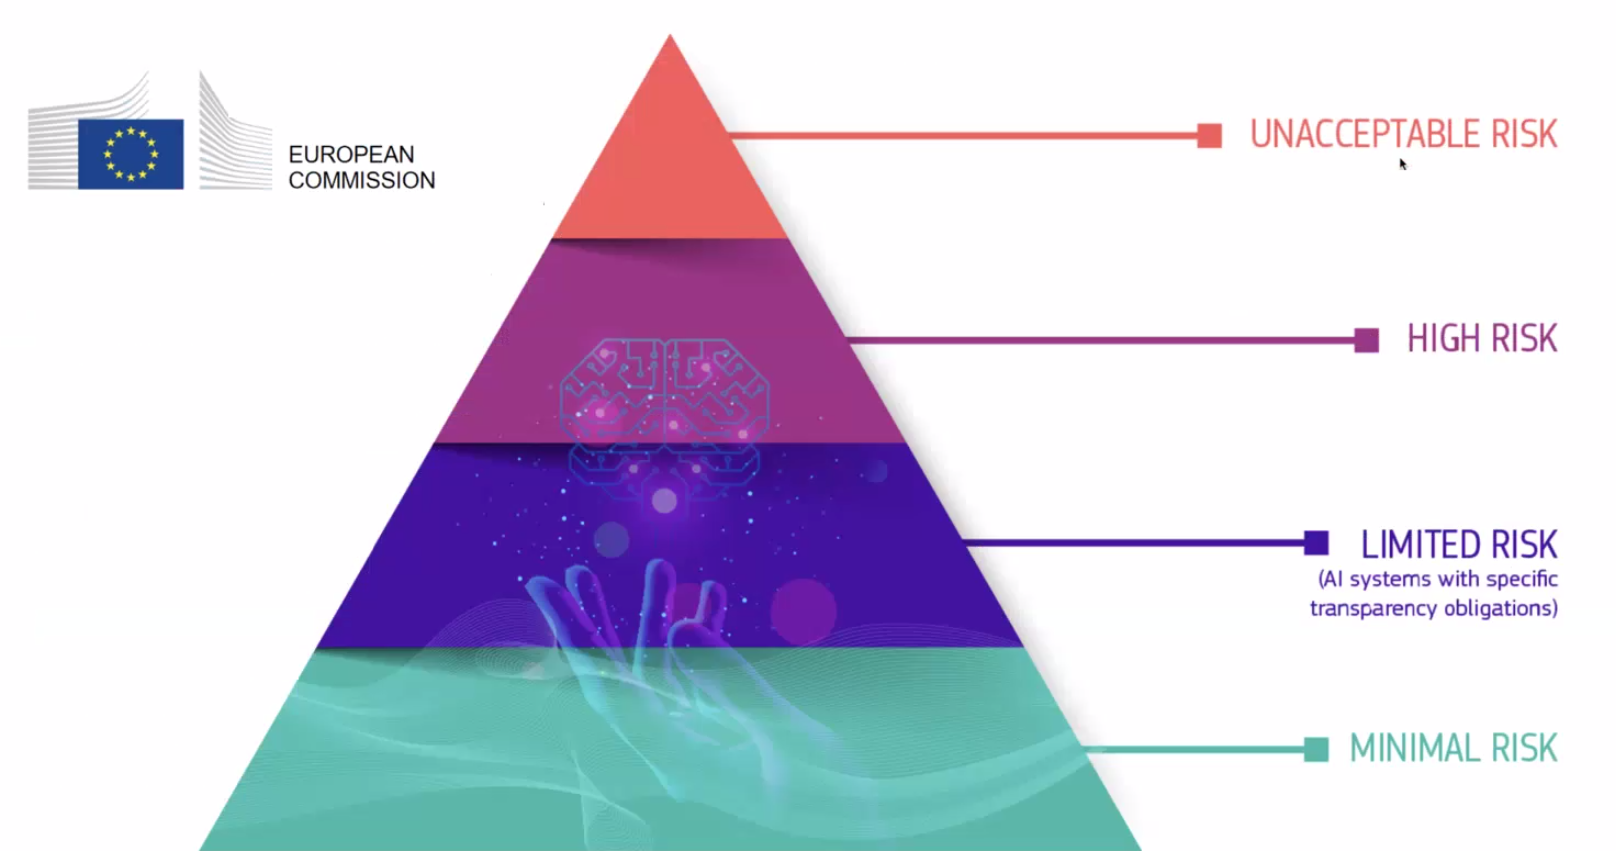
\includegraphics[width=0.8\textwidth]{paper-template/figs/risk_levels.png}
        \caption{Risk-based approach - Pyramid of risks (EU Commission, 2021) }
        \label{fig:my_label}
    \end{figure}
    Under the proposed Article 10 of the EU AI Act, an intent is not only to regulate the placing on the market of AI systems, but also to regulate the scope of training, testing, and validation data sets for AI systems that utilize machine learning.\\
    Fines for non-compliance can be as high as 6\% of global turnover for companies. The European Commission is trying to strike a balance with AI Act. On the one hand, it wants to prevent regulations from stifling innovation, and on the other hand, it wants to hinder the creation of an unrestrained AI ecosystem in Europe (also by introducing legal sandboxes that give AI developers room to maneuver). [\citet{fink2021eu}] The EU AI Act can be understood as groundbreaking in terms of the whole ecosystem. [\citet{kop2021eu}]\newline\newline
    The traffic light and traffic management system, which is currently being developed by the Fraunhofer Institute's branch for industrial automation, can be classified as a high-risk AI system (for a more detailed explanation, see below). Accordingly, the regulatory framework and the classification of systems as high-risk will be analyzed in more detail subsequently.
    Title III (Article 6) of the proposed AI Act provides a definition of what is to be classified as a high-risk AI system. It refers to systems that would have a negative impact on the safety of people or their fundamental rights. The draft law further distinguishes between two categories of high-risk AI systems.  [\citet{madiega2021artificial}] Firstly, systems with a high risk due to their use as safety components or any products that fall under the harmonization regulations of the European Union for safety and health protection. This is, for example, the use of AI in the field of toys, aviation, medical devices, passenger elevators or similar. [\citet{ebers2021standardizing}] Secondly, as described in Article 7, high-risk AI systems which are deployed one of the following: "Biometric identification and categorization of natural persons; management and operation of critical infrastructure; education and training; employment, workforce management, and access to self-employment; access to and use of essential private and government services and benefits; law enforcement; migration, asylum, and border control management; administration of justice and democratic processes." (Excerpt from Annex III of the Proposal for the EU AI Act).\\ \newline
    All of these systems that fall into the above categorization as high-risk AI systems thus have the following regulations imposed on them: \textbf{Require up-front conformity assessment:} The development of a high-risk system should ideally be done using "internal ex-ante AI Impact Assessments and Codes of Conduct overseen by inclusive, multidisciplinary teams”. [\citet{kop2021eu}]
    \textbf{Registration in the special EU database:} Providers of high-risk AI systems will be obliged to register their systems in an EU-wide database managed by the EU Commission before they launch their product on the market. \textbf{Declaration of Conformity (throughout the entire lifecycle):} The system must be approved by conformity assessment and must satisfy the corresponding requirements specified in the EU AI Act throughout its entire life cycle. Also, the Hi-Risk AI system must bear the CE marking (Conformité Européenne)\newline In addition, high-risk systems must meet other additional requirements. Specifically, they must meet requirements for "risk management, testing, technical robustness, data protection and management, transparency, human oversight, and cybersecurity" [\citet{madiega2021artificial}]as set forth in Articles 8 to 15 of the proposed EU AI Act. Not only providers, but also importers, distributors and users of AI systems must comply with these requirements. Providers with their registered office outside the EU are obliged to appoint an authorized representative within the EU who ensures conformity assessment and monitors compliance with the above-mentioned requirements and, if necessary, initiates countermeasures in the event of violations.
\newline\newline
\section*{Introduction to Fraunhofer's Automatic and Predictive Traffic Light Systems for Public Roads}
  After a detailed analysis of the EU AI Act in general and high-risk systems in particular, this paper will next analyze a system that falls into the above-mentioned category and is thus interesting for the analysis of the requirements for the system design and also for the technical implementations as well as an assessment and discussion of the risks that such a system entails.\newline
The Fraunhofer Institute, based in Munich, has been researching the use of various technical innovations in road traffic for some time in order to optimize the flow of traffic, especially in cities. A research group from the Fraunhofer Institute for Optronics, System Technologies, and Image Exploitation IOSB has recently been conducting more extensive research into the use of sensor technology around intersections, combined with the use of self-learning algorithms, in order to optimize traffic flows and achieve shorter waiting times for all road users, but above all to create improved safety for pedestrians. The research team is relying on a combination of innovative sensor technology and the use of artificial intelligence to enable "intelligent, predictive light switching." [\citet{optimized_traffic_flows_and_improved_pedestrian_safety_2022}] Presently, traffic light control in Germany is based on time-controlled and rule-based algorithms combined with the use of induction loops installed on the road surface. However, this approach only conveys a rough impression of the actual traffic situation [\citet{bmdv_2022}] and, moreover, is suitable for the constantly growing traffic volume (especially in the cities) to a limited extent only. [\citet{publisher_2022}]\newline Instead of conventional sensors, the researchers at Fraunhofer IOSB-INA employ high-resolution cameras and radar sensors to capture the actual traffic situation more accurately and are thus able to determine the exact number of waiting vehicles at an intersection in real-time and also to record and track the average speed of the cars and the waiting times of the respective vehicles.  [\citet{optimized_traffic_flows_and_improved_pedestrian_safety_2022}] The data collection serves as a foundation and input parameter for artificial intelligence, which utilizing deep reinforcement learning algorithms is able to calculate the optimal switching behavior for the traffic lights and thus create the ideal phase sequence in order to shorten the waiting times at the intersection, reduce travel times, and thus reduce the noise and CO2 pollution caused by the traffic jam. [\citet{fraunhofertrustworthy}] \newline The computational resources for the AI algorithms are provided by edge computers in the control box directly at the intersection. Looking to the future, the researchers hope for another positive advantage: the system will not only be used at individual intersections but a network of neighboring traffic lights that form a larger network can be formed with it, thus optimizing and directing the flow of traffic in real-time across larger regions. [\citet{bundesministerium_für_wirtschaft_und_klimaschutz_2022}]Initial tests, which are being conducted at an intersection in Lemgo, Germany, show that the system can generate a 10-15\% improvement in traffic flow.  [\citet{optimized_traffic_flows_and_improved_pedestrian_safety_2022}]\newline
 \begin{figure}[h]
        \centering
        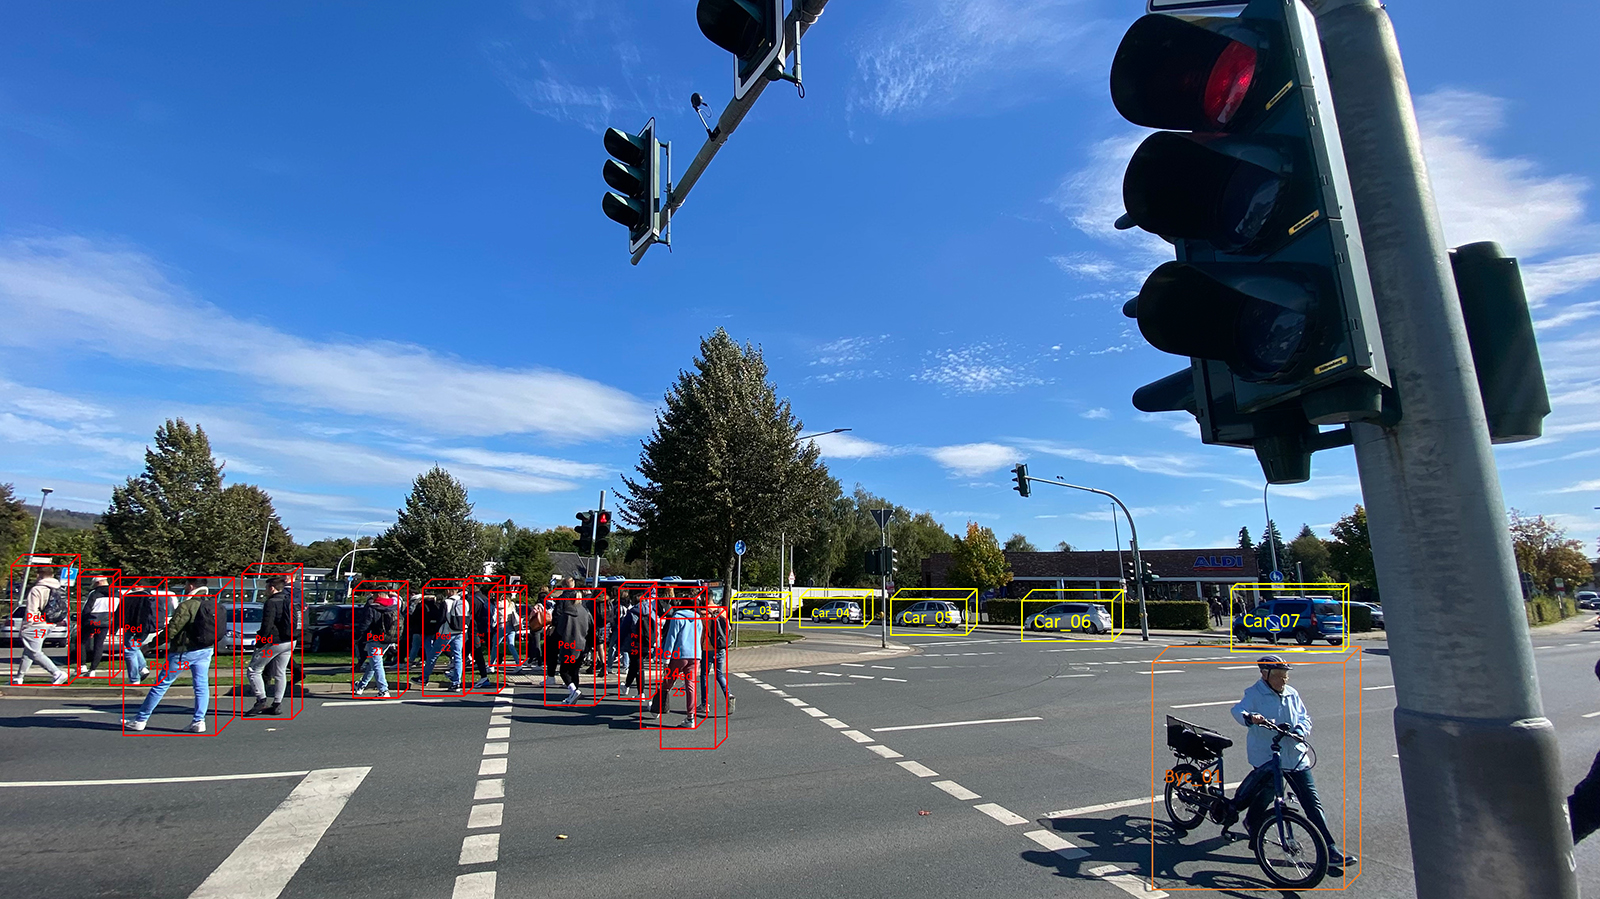
\includegraphics[width=0.8\textwidth]{paper-template/figs/traffic_lights1.jpg}
        \caption{People are detected and tracked using LiDAR sensor data and AI.}
        \label{fig:my_label}
    \end{figure}\newline
In addition to improving traffic flow, the AI-based system also aims to develop a new approach to demand-based control for pedestrian signals.  [\citet{optimized_traffic_flows_and_improved_pedestrian_safety_2022}] This is especially beneficial for vulnerable groups of people (elderly or people with disabilities). Reduce waiting times but above all increase safety at crosswalks (for example by adjusting crossing times if a person has not quite crossed the road in the time originally planned). The current solutions at traffic lights (predominantly simple buttons) are not able to meet the special needs of these groups of people. High-resolution LiDAR sensors in combination with AI can automatically adjust crossing times to the needs of pedestrians and, if necessary, extend or even shorten them to improve traffic flow at the same time. [\citet{publisher_2022}]
As a result, the research group from the Fraunhofer Institute is relying on state-of-the-art AI technology and hopes to achieve significant improvements in terms of waiting times and safety for both motorists and pedestrians with comprehensive coverage in the road network. [\citet{optimized_traffic_flows_and_improved_pedestrian_safety_2022}] The research area is divided into the two research projects KI4LSA and KI4PED, which focus on motor vehicle traffic and pedestrian traffic, respectively.\newpage
 \begin{figure}[h]
        \centering
        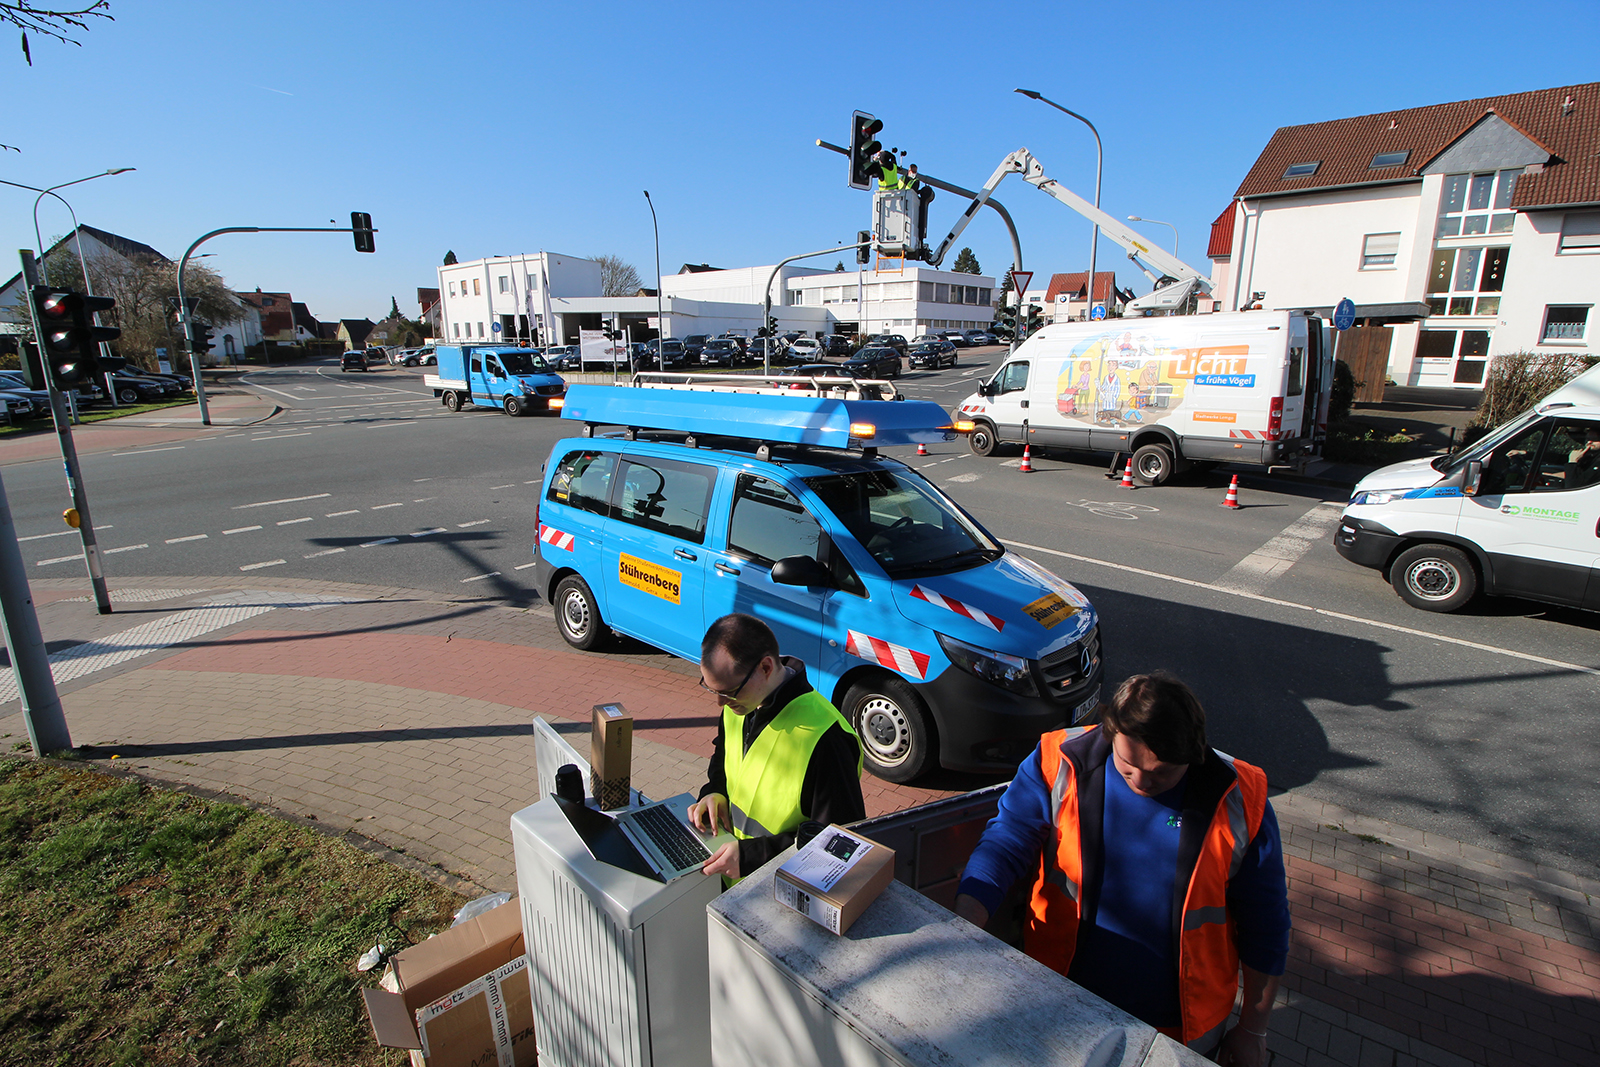
\includegraphics[width=0.8\textwidth]{paper-template/figs/traffic_light2.jpg}
        \caption{Highresolution cameras and radar sensors gather detailed traffic information.}
        \label{fig:my_label}
    \end{figure}
 \textbf{Why Fraunhofer's traffic light system should be classified as a high-risk AI tool}\newline In the previous paragraphs, a general analysis of high-risk systems, including the definition and an explanation of when an AI system is considered a high-risk AI system, has already been presented. The question, which remains unanswered so far, is whether the Fraunhofer Institute's traffic light system that has just been explained falls into the categorization of a high-risk AI System as it is lied down in the proposal of the EU AI Act.\newline
As stated in Article 6 f of the European Commission's proposal for the EU AI Act, any system is to be classified as high-risk if it is included in the list of Annex III. This includes all systems that are used in the management or operation of critical infrastructure. [\citet{madiega2021artificial}]  Use in critical infrastructure here includes, above all, all AI systems that are to be used as safety components for the management and operation of road traffic as well as water, gas, heat, and electricity supplies. \newline
Since Fraunhofer's Traffic Light System is evidently an operation within road traffic, Article 6 f necessarily applies - especially since it is clearly also intended to be used on public roads. Thus, the Traffic Light Systems might clearly be considered a high-risk AI system. 
However, the classification seems to be trivial only at first glance, since currently the technical implementation is being developed towards finding a two-layer system that fulfills additional security standards. By adding an additional security layer, this system could possibly be classified as a limited-risk system after all. Technically, it is implemented by the AI system calculating in the background making requests to the safety layer (for example, the request to switch the traffic light from red to green) with the safety layer comparing the request with existing safety parameters (such as specific time intervals between green phases, etc.) and thus there is no longer a purely AI-based control of traffic, but merely a proposing  AI part to it, which is limited by safety mechanisms. [\citet{seick}] Since this system is currently still under development, this additional technical component is excluded for the time being and the system is classified as high-risk.\newline
Therefore, if the system is to be used on roads within the EU, this will also entail the obligations mentioned in Part 1 relating to the development, use, and commercialization of such a system.
